\documentclass[tikz,border=8pt]{standalone}
\usepackage{tikz}
\usetikzlibrary{positioning,arrows.meta,shapes.geometric,fit,backgrounds,calc}
\usepackage{fontspec}
\setmainfont{Times New Roman}

\begin{document}
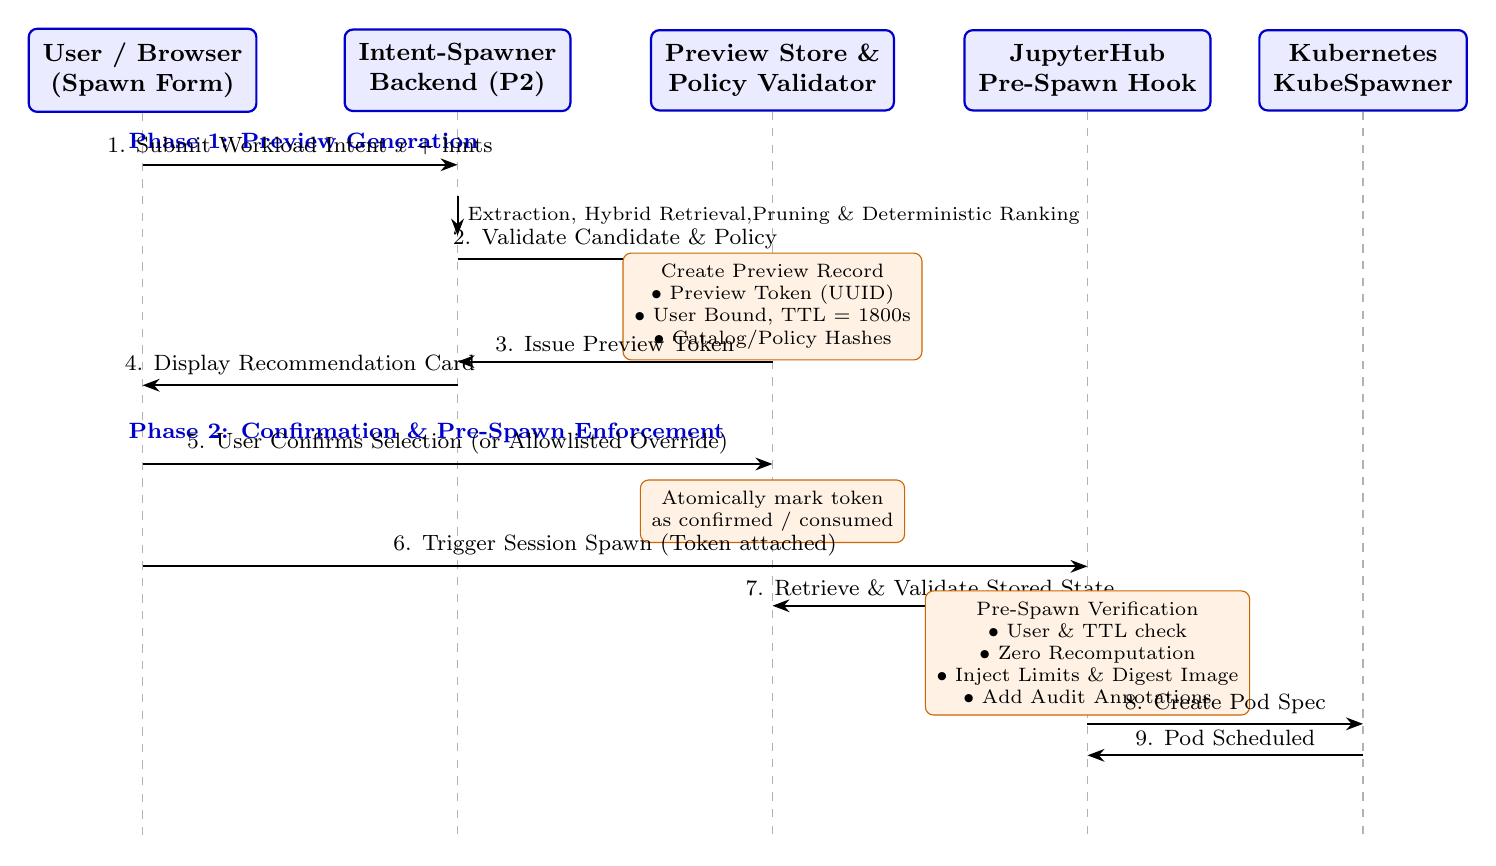
\begin{tikzpicture}[
    font=\small,
    >=Stealth,
    actor/.style={
        draw=blue!80!black,
        fill=blue!8,
        rounded corners=3pt,
        align=center,
        line width=0.8pt,
        inner sep=5pt,
        minimum width=2.4cm,
        minimum height=0.8cm,
        font=\small\bfseries
    },
    lifeline/.style={
        draw=gray!60,
        dashed,
        line width=0.6pt
    },
    msg/.style={
        ->,
        line width=0.7pt,
        font=\footnotesize
    },
    note/.style={
        draw=orange!80!black,
        fill=orange!10,
        rounded corners=3pt,
        font=\scriptsize,
        inner sep=4pt,
        align=center
    }
]

% Actors
\node[actor] (user) at (0,0) {User / Browser\\(Spawn Form)};
\node[actor] (p2) at (4.0,0) {Intent-Spawner\\Backend (P2)};
\node[actor] (preview) at (8.0,0) {Preview Store \&\\Policy Validator};
\node[actor] (hook) at (12.0,0) {JupyterHub\\Pre-Spawn Hook};
\node[actor] (k8s) at (15.5,0) {Kubernetes\\KubeSpawner};

% Lifelines
\draw[lifeline] (user.south) -- ++(0, -9.2) coordinate (user_end);
\draw[lifeline] (p2.south) -- ++(0, -9.2) coordinate (p2_end);
\draw[lifeline] (preview.south) -- ++(0, -9.2) coordinate (preview_end);
\draw[lifeline] (hook.south) -- ++(0, -9.2) coordinate (hook_end);
\draw[lifeline] (k8s.south) -- ++(0, -9.2) coordinate (k8s_end);

% Phase 1: Preview Generation
\node[anchor=west, font=\footnotesize\bfseries\color{blue!80!black}] at (-0.3, -0.9) {Phase 1: Preview Generation};
\draw[msg] (0, -1.2) -- (4.0, -1.2) node[midway, above] {1. Submit Workload Intent $x$ + hints};
\draw[msg] (4.0, -1.6) -- (4.0, -2.1) node[midway, right, font=\scriptsize] {Extraction, Hybrid Retrieval,\\Pruning \& Deterministic Ranking};
\draw[msg] (4.0, -2.4) -- (8.0, -2.4) node[midway, above] {2. Validate Candidate \& Policy};
\node[note] at (8.0, -3.0) {Create Preview Record\\$\bullet$ Preview Token (UUID)\\$\bullet$ User Bound, TTL = 1800s\\$\bullet$ Catalog/Policy Hashes};
\draw[msg] (8.0, -3.7) -- (4.0, -3.7) node[midway, above] {3. Issue Preview Token};
\draw[msg] (4.0, -4.0) -- (0, -4.0) node[midway, above] {4. Display Recommendation Card};

% Phase 2: Confirmation & Spawning
\node[anchor=west, font=\footnotesize\bfseries\color{blue!80!black}] at (-0.3, -4.6) {Phase 2: Confirmation \& Pre-Spawn Enforcement};
\draw[msg] (0, -5.0) -- (8.0, -5.0) node[midway, above] {5. User Confirms Selection (or Allowlisted Override)};
\node[note] at (8.0, -5.6) {Atomically mark token\\as confirmed / consumed};
\draw[msg] (0, -6.3) -- (12.0, -6.3) node[midway, above] {6. Trigger Session Spawn (Token attached)};
\draw[msg] (12.0, -6.8) -- (8.0, -6.8) node[midway, above] {7. Retrieve \& Validate Stored State};
\node[note] at (12.0, -7.4) {Pre-Spawn Verification\\$\bullet$ User \& TTL check\\$\bullet$ Zero Recomputation\\$\bullet$ Inject Limits \& Digest Image\\$\bullet$ Add Audit Annotations};
\draw[msg] (12.0, -8.3) -- (15.5, -8.3) node[midway, above] {8. Create Pod Spec};
\draw[msg] (15.5, -8.7) -- (12.0, -8.7) node[midway, above] {9. Pod Scheduled};

\end{tikzpicture}
\end{document}
